\setAuthor{Tundmatu autor}
\setRound{lahtine}
\setYear{2004}
\setNumber{G 7}
\setDifficulty{5}
\setTopic{Elektrostaatika}

\prob{Laetud numbrilaud}
Kella numbrilauale on fikseeritud punktlaengud suurusega $q, 2q, 3q, \ldots, 12q$ ($q > 0$), mis paiknevad vastavatel tunnijaotistel. Millist aega näitab tunniosuti hetkel, kui ta on paralleelne ja samasuunaline nende laengute poolt tekitatud resultantväljatugevuse vektoriga numbrilaua tsentris?

\hint
Paneme tähele, et summaarne laengute poolt tekitatud elektriväli on individuaalsete laengute tekitatud elektriväljade summa (kus elektriväljad on vektoriaalselt kokku liidetud). Ülesannet lihtsustab oluliselt laengute kokku liitmise järjekord, näiteks on mugav laengute panuseid diagonaale järgi paarikaupa kokku arvestada.

\solu
Iga laeng $nq$ tekitab numbrilaua tsentris välja, mille moodul on võrdeline $nq$-ga ja mis on suunatud radiaalselt laengust eemale. Vektorite liitmise järjekord pole oluline, seega võime sümmeetria tõttu esmalt liita paarikaupa samal diagonaalil paiknevate laengute väljad. Sellest ideest lähtuvalt näeme, et algne konfiguratsioon on ekvivalentne laengute lihtsama paigutusega (vt. joon. 2). Nüüd on sümmeetria põhjal kerge näha, et resultantvälja vektor osutab kellaajale 3.30.
\begin{center}
	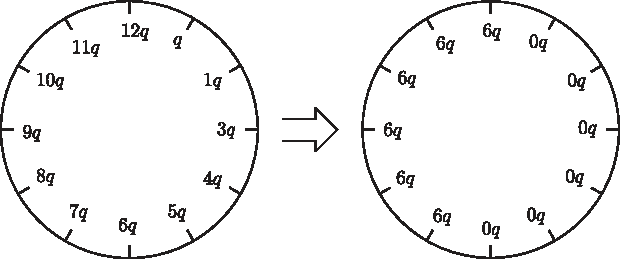
\includegraphics[width=0.7\linewidth]{2004-lahg-07-lah.pdf}
\end{center}
\probend